\documentclass[conference]{IEEEtran}
\IEEEoverridecommandlockouts%
% The preceding line only needs to identify funding in the first footnote. If that is unnecessary, please comment on it.
\usepackage{cite}
\usepackage{amsmath,amssymb,amsfonts}
\usepackage{algorithmic}
\usepackage{graphicx}
\usepackage{textcomp}
\usepackage{xcolor}
\usepackage{hyperref}
\usepackage{caption}
\usepackage{comment}
\usepackage{colortbl}
\usepackage{booktabs}
\usepackage{tabularx}
\usepackage[most]{tcolorbox}
\usepackage{pdfpages}

\newenvironment{bgquote} {\begin{tcolorbox}[ enhanced, breakable=true, colback=blue!5, colframe=white, boxrule=0pt, left=1em, right=1em, top=0.5em, bottom=0.5em, boxsep=0pt, width=\linewidth, before skip=0.5em, after skip=0.5em ]} {\end{tcolorbox}}

\def\BibTeX{{\rm B\kern-.05em{\sc i\kern-.025em b}\kern-.08em
    T\kern-.1667em\lower.7ex\hbox{E}\kern-.125emX}}

\begin{document}

\title{Deep Learning Lab 5 \\
%{\footnotesize \textsuperscript{*}Note: Subtitles should not be used}
}

\author{\IEEEauthorblockN{Suraj Karki}
\IEEEauthorblockA{\textit{Department of Engineering Science }\\
\textit{University West}\\
Trollhättan, Sweden \\
suraj.karki@student.hv.se}
\and
\IEEEauthorblockN{Nils Karlsson}
\IEEEauthorblockA{\textit{Department of Engineering Science }\\
\textit{University West}\\
Trollhättan, Sweden \\
nils.Karlsson@student.hv.se}
\and
\IEEEauthorblockN{Nils Wikström}
\IEEEauthorblockA{\textit{Department of Engineering Science} \\
\textit{University West}\\
Trollhättan, Sweden \\
nils.wikstrom@student.hv.se}
}

\maketitle

\thispagestyle{plain}
\pagestyle{plain}


\begin{IEEEkeywords}
Deep Learning, Laboration 5, CNN 
\end{IEEEkeywords}
\begin{abstract}
    The source code for this lab can be found at\cite{dataset}. 
\end{abstract}

\section{Task 1}
\subsection{Apply convolution on a custom image and show the results.}
First, we constructed a custom image of size $70 \times 120$ with three colour channels (RGB). 
The image was extracted from a sample dataset, centre-cropped to the required spatial dimensions, 
and rescaled to the interval $[0,1]$ for numerical stability during convolution.

Figure~\ref{fig:custom_image} shows the custom images after preprocessing.

\begin{figure}[ht]
    \centering
    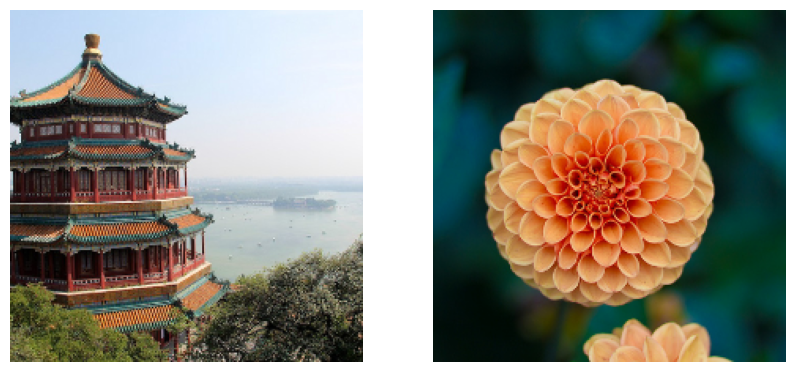
\includegraphics[width=0.48\textwidth]{figures/Origianl_image.png} 
    \caption{Custom image 1 after preprocessing.}\label{fig:custom_image}
\end{figure}


Then we applied convolution layer with 32 filters and a kernel size of $7 \times 7$ on the custom images. Figure~\ref{fig:convolution_result} shows the result of applying convolution on custom images. The convolution layer was able to extract features from the images, which can be used for further processing in a neural network.

\begin{figure}[ht]
    \centering
    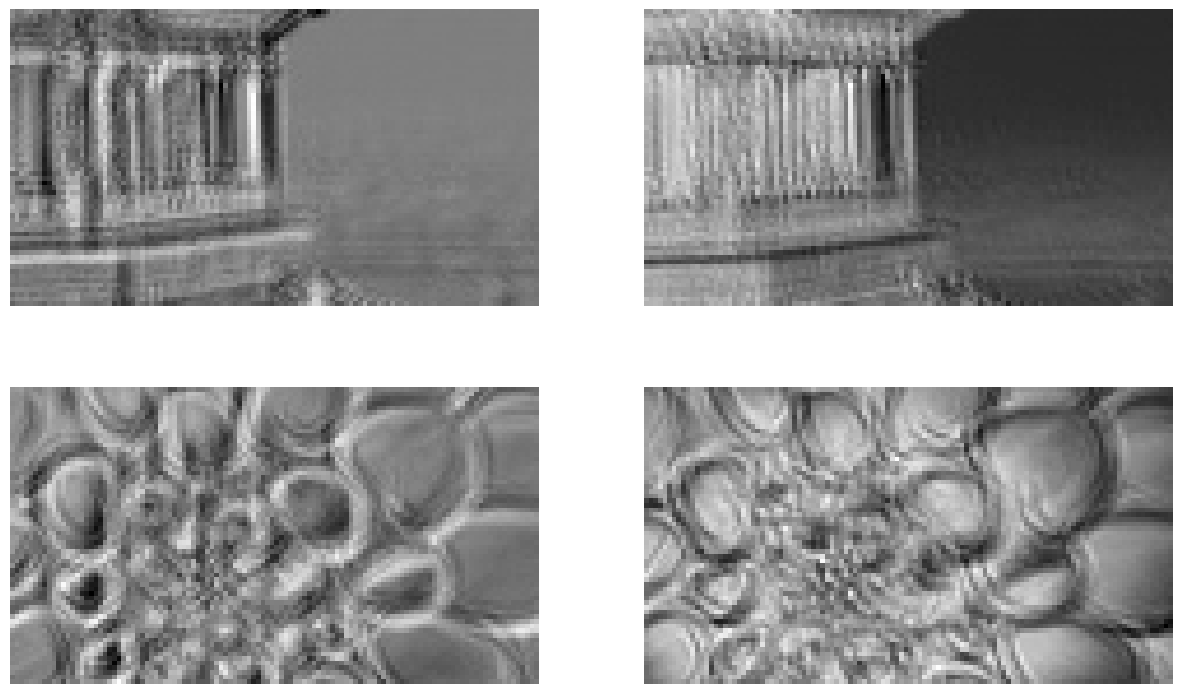
\includegraphics[width=0.48\textwidth]{figures/result_of_applying_convolution.png} 
    \caption{Result of applying convolution on custom images.}\label{fig:convolution_result}
\end{figure}

\subsection{Apply max-pooling, depth-wise pooling, and average pooling on the images from the previous step and show the results.}
We applied max-pooling, depth-wise pooling, and average pooling on the convolution result from the previous step. Figure~\ref{fig:poolingResult}, Figure~\ref{fig:averagePoolingResult}, and Figure~\ref{fig:depthwise_pooling_result} shows the first feautre map of applying different pooling techniques to the convolution result. Max-pooling takes the maximum value from each patch of the feature map, while average pooling takes the average value. Depth-wise pooling is a type of pooling that operates on each channel separately. The pooling layers help to reduce the spatial dimensions of the feature maps while retaining important features, which can improve the performance of the neural network.
\begin{figure}[ht]
    \centering
    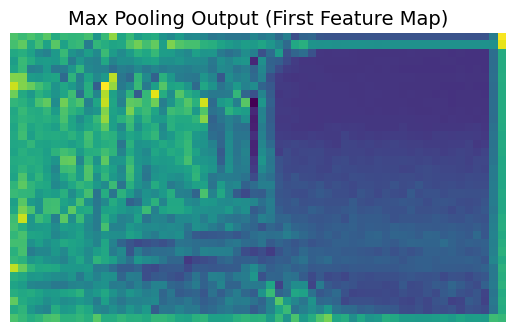
\includegraphics[width=0.48\textwidth]{figures/pollingResult.png} 
    \caption{Result of applying max-pooling on the convolution result.}\label{fig:poolingResult}
\end{figure}
\begin{figure}[ht]
    \centering
    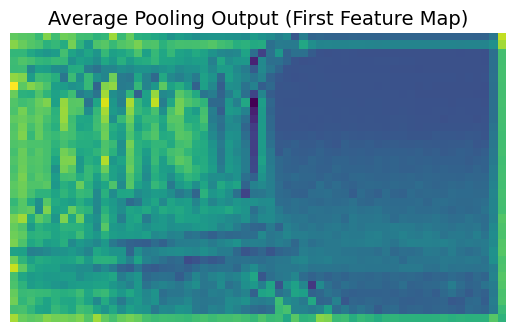
\includegraphics[width=0.48\textwidth]{figures/pooling_result1.png} 
    \caption{Result of applying average pooling on the convolution result.}\label{fig:averagePoolingResult}
\end{figure}

\begin{figure}[ht]
    \centering
    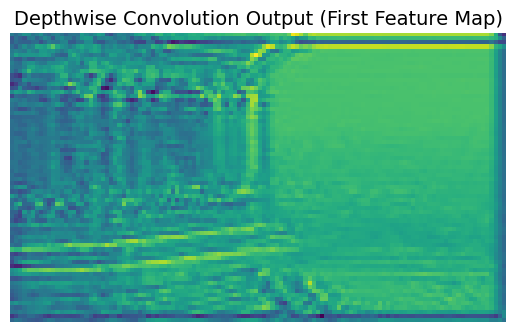
\includegraphics[width=0.48\textwidth]{figures/depthWisePooling.png} 
    \caption{Result of applying depth-wise pooling on the convolution result.}\label{fig:depthwise_pooling_result}
\end{figure}


\section{Task 2- Create and train a convolutional neural network for the MNIST Fashion dataset and compare the results of the CNN and FCN.}
In previous lab, a Fully Connected Network (FCN) was implemented for the classification of the Fashion MNIST dataset. 
While FCNs treat images as flattened vectors and ignore spatial structure, Convolutional Neural Networks (CNNs) explicitly exploit local spatial correlations through convolutional filters and pooling operations. This typically leads to improved generalisation performance and greater parameter efficiency.

Although FCNs are capable of learning non-linear decision boundaries, they treat input images as flattened vectors, thereby discarding spatial structure. In contrast, CNNs leverage convolutional filters to capture local spatial features such as edges and textures, and pooling layers to achieve translation invariance.

The CNN consists of multiple convolutional layers organised into hierarchical blocks. 
Each convolutional layer applies learnable filters that extract local spatial features such as edges, textures, and object parts. 
ReLU activation functions introduce non-linearity, while He initialisation ensures stable gradient propagation during training.

Max pooling layers are inserted between convolutional blocks to reduce spatial dimensions. 
This downsampling operation provides translation invariance and reduces computational complexity. 
As the network depth increases, the number of filters is increased, allowing the model to capture progressively more abstract representations.

After the convolutional feature extraction stage, the feature maps are flattened and passed through fully connected layers. 
Dropout regularisation is applied to mitigate overfitting by randomly deactivating neurons during training. 
Finally, a softmax output layer produces probability distributions over the ten Fashion MNIST classes. Figure~\ref{fig:cnn_result} illustrates the result from single conv layer CNN.

\begin{figure*}[ht]
    \centering
    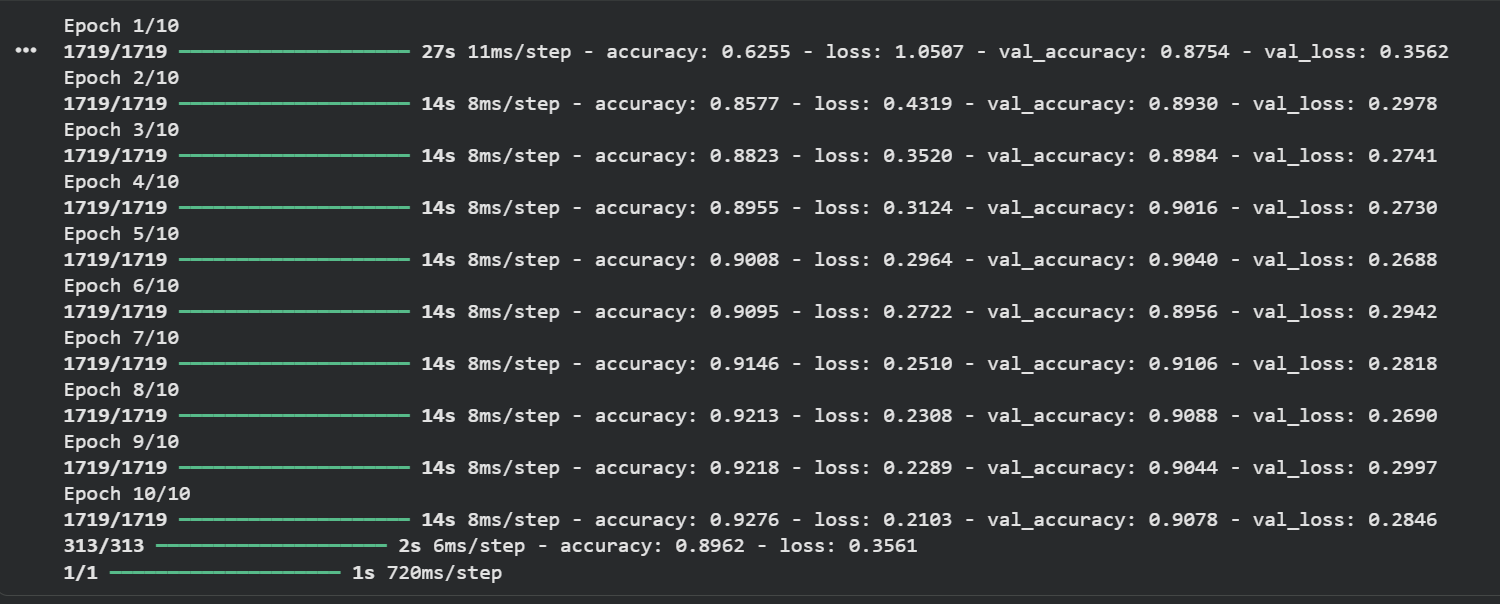
\includegraphics[width=\textwidth]{figures/mnist_cnn_result.png} 
    \caption{Result of training the CNN on Fashion MNIST dataset.}\label{fig:cnn_result}
\end{figure*}

For further experimentation, another cnn architecturre was implemented with more convolutional layers combining the FCN. The results of the second CNN architecture are shown in Figure~\ref{fig:cnn_result2}. The second CNN architecture achieved over 99\% accuracy, demonstrating the importance of architectural design.

\begin{itemize}
    \item \textbf{Convolutional Layers:}  
    Two convolutional layers were used:
    \begin{enumerate}
        \item The first layer applies 32 filters of size $3 \times 3$ with \texttt{same} padding, followed by a ReLU activation.  
        \item The second layer applies 64 filters of size $3 \times 3$, also with \texttt{same} padding and ReLU activation.
    \end{enumerate}
    These layers extract low- to mid-level spatial features such as edges, textures, and simple patterns.
    
    \item \textbf{Max Pooling:} To reduce the spatial dimensions of the feature maps.
    
    \item \textbf{Flattening:}  
    The multi-dimensional feature maps are flattened into a 1D vector, preparing the data for fully connected layers.
    
    \item \textbf{Fully Connected Layers and Dropout:}  
    The first dense layer has 128 units with ReLU activation, followed by a dropout of 25\% to reduce overfitting.  
    The second dense layer acts as the output layer with 10 units corresponding to the 10 Fashion MNIST classes and a softmax activation to produce probability distributions. An additional dropout of 50\% is applied before the output.
\end{itemize}

\begin{figure*}[ht]
    \centering
    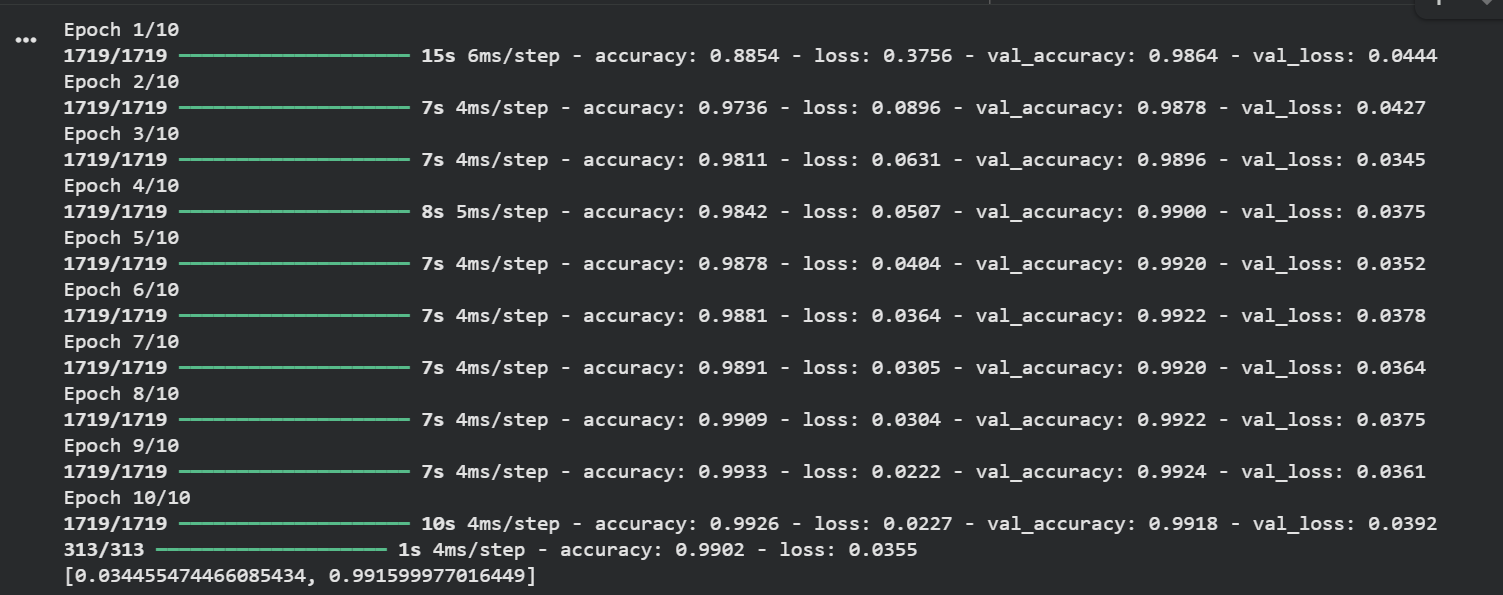
\includegraphics[width=\textwidth]{figures/cnn_result2.png} 
    \caption{Result of training the second CNN architecture on Fashion MNIST dataset (2 conv layer).}\label{fig:cnn_result2}
\end{figure*}



\section{Task 3- Implement a ResNet-34 CNN model using Keras}
ResNet (Residual Network) introduces identity-based skip connections to address the degradation problem observed in very deep neural networks~\cite{resnet34}. Instead of learning a direct mapping $H(x)$, each residual block learns a residual function:

\[
F(x) = H(x) - x
\]

The output of a residual unit is therefore defined as:

\[
y = F(x) + x
\]

This resnet facilitates gradient flow during backpropagation and mitigates vanishing gradient issues, enabling the successful training of substantially deeper architectures~\cite{resnet34}.
Each residual unit consists of two convolutional layers with $3 \times 3$ kernels, followed by batch normalisation. A ReLU activation function is applied after the first convolution and after the residual addition.

The structure of the main branch is:

\[
\text{Conv} \rightarrow \text{BatchNorm} \rightarrow \text{ReLU} \rightarrow \text{Conv} \rightarrow \text{BatchNorm}
\]

When spatial dimensions or channel depth change (i.e.\ when stride $>1$), a $1 \times 1$ convolution is applied in the skip branch to match dimensions before addition. Otherwise, the skip connection acts as an identity mapping.

He initialisation is used for all convolutional layers to ensure stable variance propagation in deep networks.
The model follows the canonical ResNet-34 configuration:

\[
[64] \times 3,\quad
[128] \times 4,\quad
[256] \times 6,\quad
[512] \times 3
\]

Summary of the archetecture:

\begin{itemize}
    \item Initial $7 \times 7$ convolution with stride 2
    \item Batch normalisation and ReLU activation
    \item $3 \times 3$ max pooling
    \item 16 residual units organised in four stages
    \item Global average pooling
    \item Fully connected softmax layer with 10 outputs
\end{itemize}

Global average pooling replaces traditional dense layers, significantly reducing the number of parameters and improving generalisation.
The model was trained on the Fashion MNIST dataset. The network was compiled using:

\begin{itemize}
    \item Loss function: Sparse categorical cross-entropy
    \item Optimiser: Nadam
    \item Evaluation metric: Accuracy
\end{itemize}

Training was conducted for 10 epochs using a validation split. Model performance was subsequently evaluated on the held-out test set.

The ResNet-34 architecture achieved high classification accuracy on the Fashion MNIST dataset. Compared to earlier experiments:
Figure~\ref{fig:resnet34_training} and Figure~\ref{fig:resnet34_epoch} demonstrates the training and validation accuracy for the ResNet-34 model.
\begin{figure*}[ht]
    \centering
    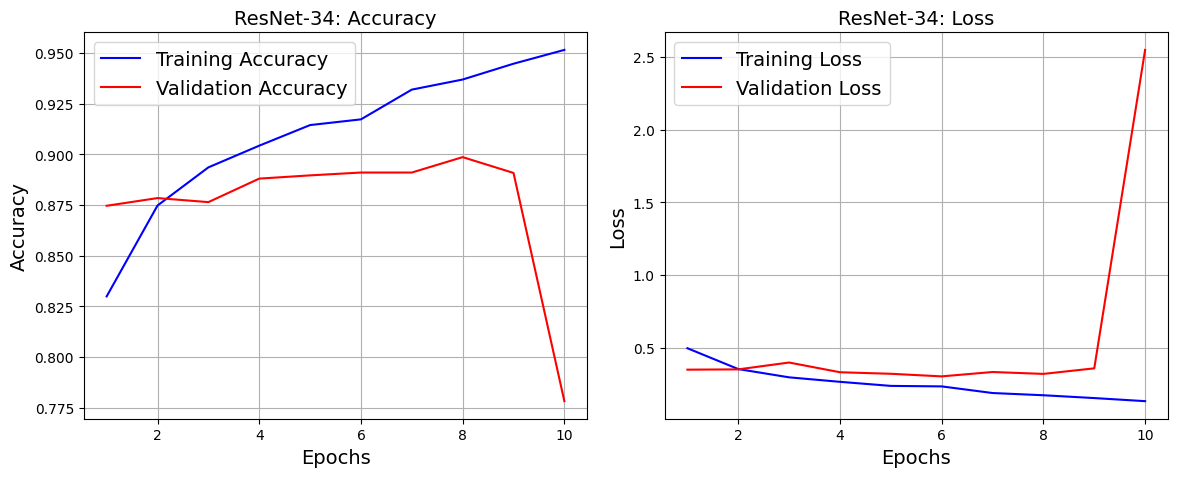
\includegraphics[width=\textwidth]{figures/resnet_accuracyAndLoss.png} 
    \caption{Training and validation accuracy for ResNet-34 model on Fashion MNIST dataset.}\label{fig:resnet34_training}
\end{figure*}

\begin{figure*}[ht]
    \centering
    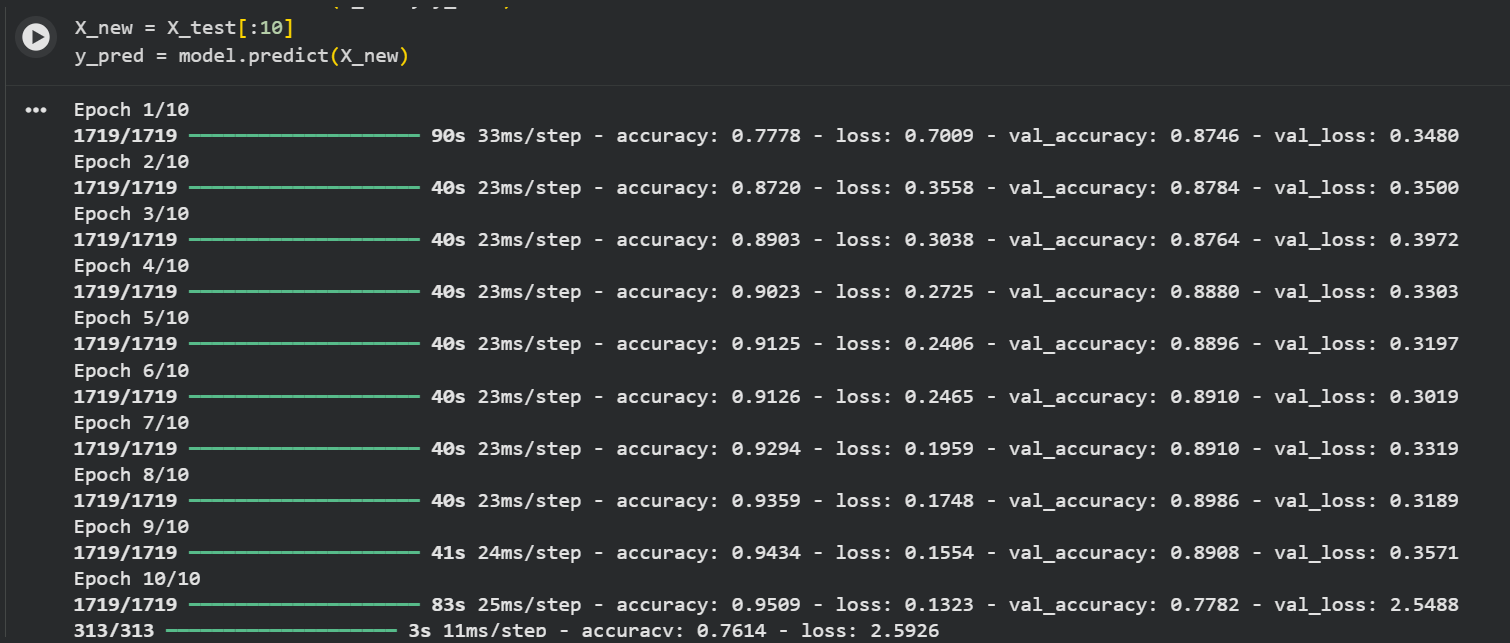
\includegraphics[width=\textwidth]{figures/resnet_trainingandevaluation.png} 
    \caption{Training and evaluation results each epoch.}\label{fig:resnet34_epoch}
\end{figure*}

\section{Task 4- Use a pre-trained Xception model for transfer learning.}In this task, we implemented a convolutional neural network using a pre-trained \texttt{Xception} model from \texttt{Keras Applications} and applied it to a new classification task to TF Flowers dataset. Transfer learning allows leveraging features learned from large-scale datasets such as ImageNet and applying them to smaller, domain-specific datasets, improving training efficiency and performance.


\subsection{Load a dataset (e.g., tf\_flowers) and split it into training, validation, and testing datasets}
The dataset was split into training, validation, and testing sets as follows. 

\begin{itemize}
    \item \texttt{train[:10\%]} – first 10\% of the dataset, used as the \textbf{test set}.
    \item \texttt{train[10\%:25\%]} – next 15\% of the dataset, used as the \textbf{validation set}.
    \item \texttt{train[25\%:]} – remaining 75\% of the dataset, used as the \textbf{training set}.
\end{itemize}

\subsection{Pre-process and resize the images.}
Figure~\ref{fig:dataset} shows sample images from the tf\_flowers dataset after preprocessing. The images were resized to $224 \times 224$ pixels, which is the input size required by the Xception model.
\begin{figure}[ht]
    \centering
    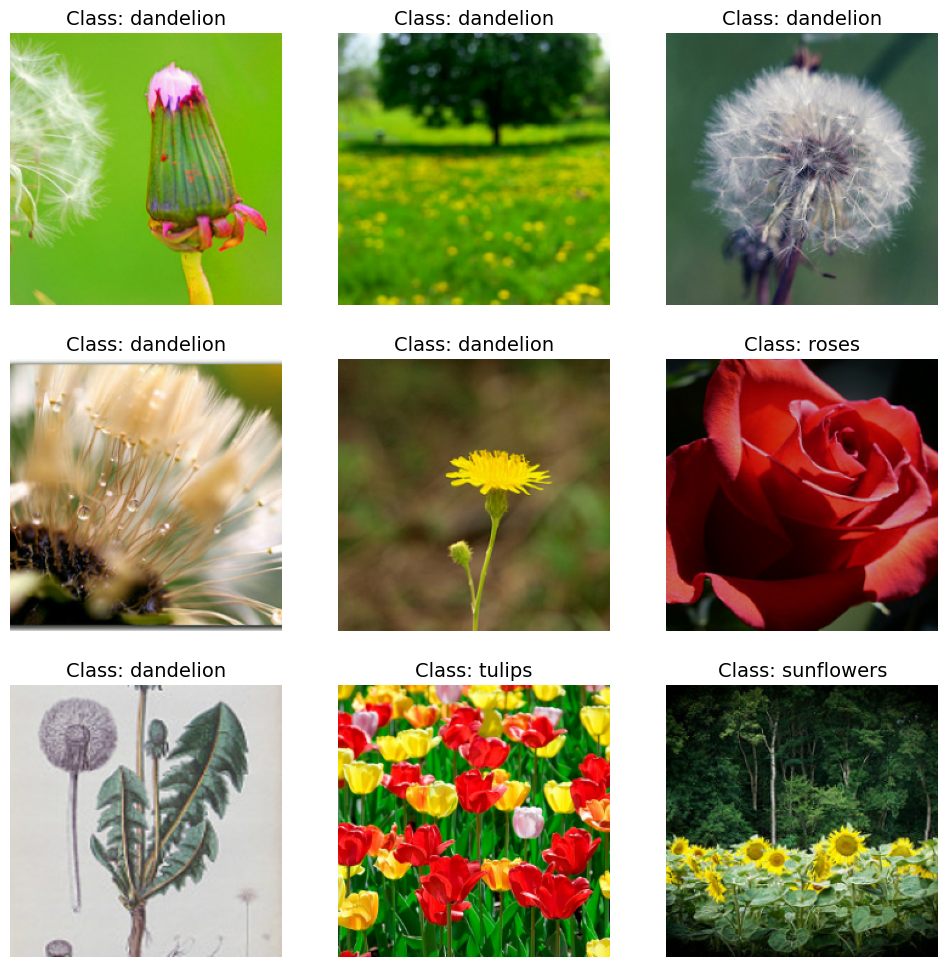
\includegraphics[width=0.48\textwidth]{figures/dataset.png} 
    \caption{first 9 images from the tf\_flowers dataset.}\label{fig:dataset}
\end{figure}

\subsection{Create the Keras model and freeze the weights of the pre-trained layers.}

The Xception model, which is based on depthwise separable convolutions, was loaded with the following configuration:
\begin{itemize}
    \item \textbf{Pre-trained Weights:} The model was initialised with \texttt{imagenet} weights, allowing it to reuse features learned on over one million images across 1000 classes.
    \item \textbf{Top Layer Exclusion:} The fully connected top layer (\texttt{include\_top=False}) was removed to enable the addition of a custom classifier suitable for this tf\_flowers dataset.
    \item \textbf{Global Average Pooling:} A \texttt{GlobalAveragePooling2D} layer was applied to the output feature maps of the base model. This reduces each feature map to a single value, converting the 2D spatial data into a 1D feature vector suitable for dense layers.
    \item \textbf{Custom Output Layer:} A dense layer with \texttt{softmax} activation was added as the output layer, with the number of units corresponding to the number of classes (\texttt{n\_classes}) in the new dataset.
\end{itemize}

To preserve the knowledge learned on ImageNet and prevent it from being overwritten during training on this dataset, all layers of the pre-trained Xception base were frozen:

\begin{itemize}
    \item Each layer in \texttt{base\_model.layers} was set to \texttt{trainable = False}.
    \item Only the custom output layer is trainable, allowing the network to learn task-specific class mappings while preserving the pre-trained features.
\end{itemize}


\subsection{Train the model and report the results.}
Figure~\ref{fig:transfer_learning_result} and Figure~\ref{fig:transfer_learning_plot} demonstrates the training and validation accuracy and loss for the transfer learning model using the pre-trained Xception architecture. The model was trained for 10 epochs, and the results indicate that transfer learning significantly improved performance compared to training a model from scratch on this dataset.
\begin{figure*}[ht]
    \centering
    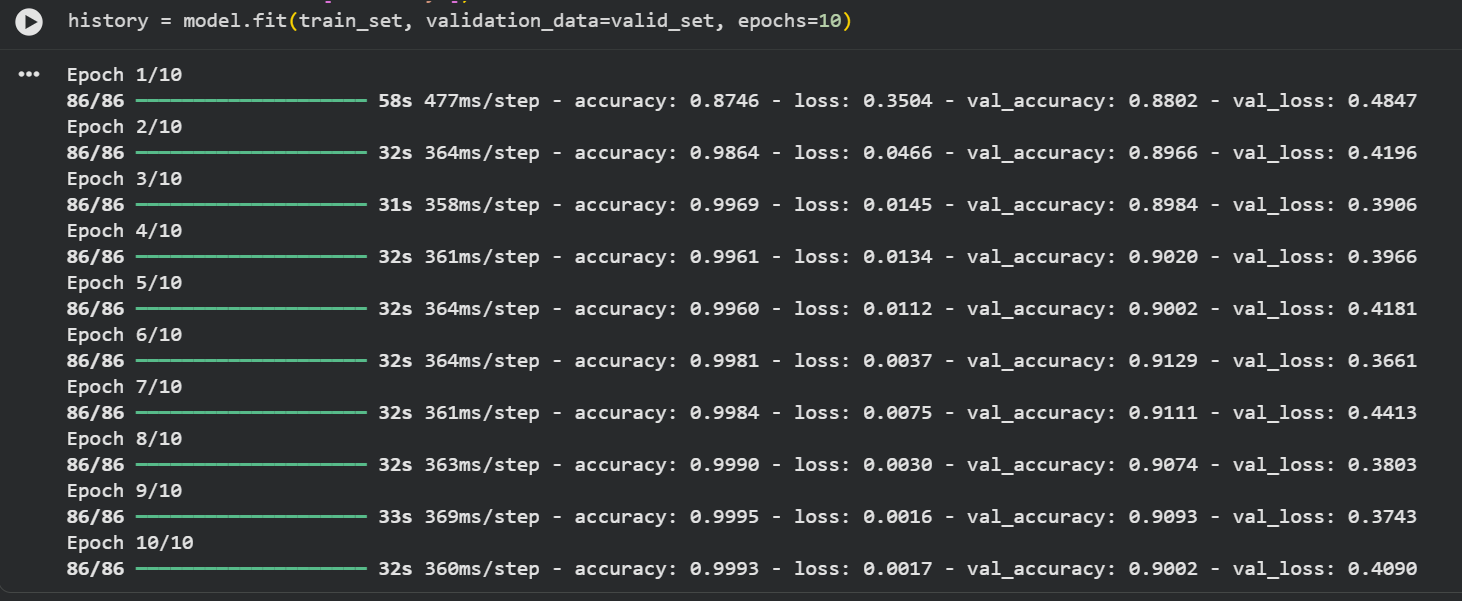
\includegraphics[width=\textwidth]{figures/xception_training.png} 
    \caption{Training and validation accuracy for the transfer learning model using pre-trained Xception architecture.}\label{fig:transfer_learning_result}
\end{figure*}
\begin{figure*}[ht]
    \centering
    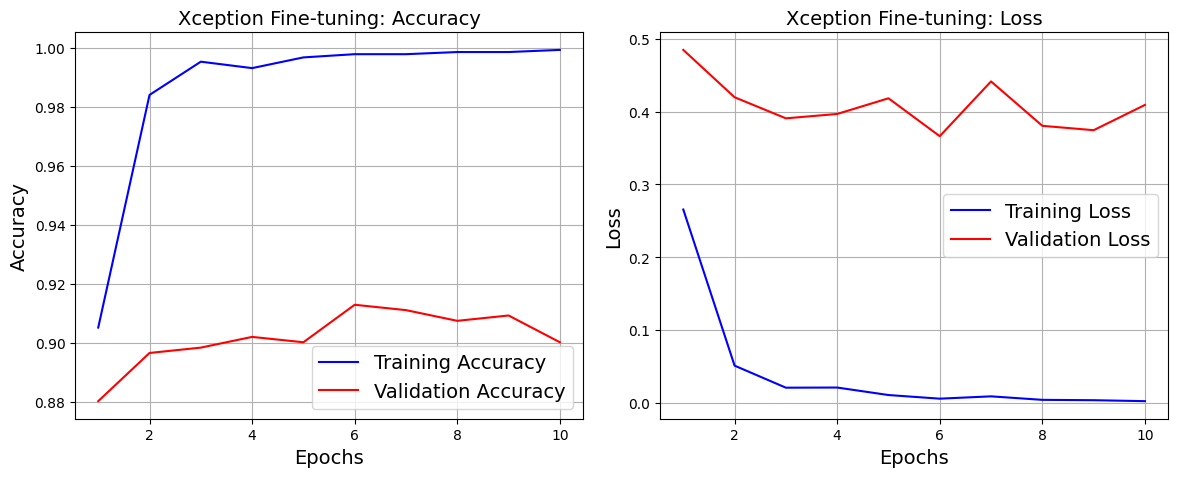
\includegraphics[width=\textwidth]{figures/xception_result.png} 
    \caption{Training and validation accuracy for the transfer learning model using pre-trained Xception architecture.}\label{fig:transfer_learning_plot}
\end{figure*}

\bibliographystyle{IEEEtran}
\bibliography{references}

%\textbf{Important for each reference is that it is a clickable doi that makes it easy for a reader to get hold of the reference directly (see examples in bib file).}

\end{document}


